% Pitch de 6 minutos - Radar Tutor UC
% Compilar con XeLaTeX:  xelatex Pitch.tex
\documentclass[aspectratio=169,10pt]{beamer}

\usepackage{fontspec}
\setsansfont{Open Sans}
\usepackage[spanish,es-noquoting]{babel}
\usepackage{tikz}
\usepackage{tcolorbox}
\usepackage{fontawesome5}
\usepackage{booktabs}

% ---------- Colores y estilo
\definecolor{azul}{HTML}{1F4E79}
\definecolor{azulclaro}{HTML}{E8F1FB}
\definecolor{rojo}{HTML}{D62728}
\definecolor{ambar}{HTML}{E0A800}
\definecolor{verde}{HTML}{2CA02C}
\definecolor{gris}{HTML}{5B6775}
\definecolor{fondo}{HTML}{F4F6F9}

\setbeamercolor{normal text}{fg=black!85}
\setbeamercolor{structure}{fg=azul}
\setbeamercolor{alerted text}{fg=rojo}
\setbeamerfont{frametitle}{size=\Large,series=\bfseries}
\setbeamertemplate{navigation symbols}{}
\setbeamertemplate{itemize items}{\textcolor{azul}{\raisebox{1pt}{\scriptsize$\blacktriangleright$}}}
\setbeamertemplate{enumerate items}[circle]

% Etiqueta de sección y tiempo (estructura fija del pitch)
\newcommand{\bloque}{}
\newcommand{\setbloque}[1]{\renewcommand{\bloque}{#1}}

\setbeamersize{text margin left=0.55cm,text margin right=0.55cm}
\setbeamertemplate{frametitle}{%
  \begin{tikzpicture}[remember picture,overlay]
    \fill[azul] (current page.north west) rectangle ([yshift=-1.15cm]current page.north east);
    \node[anchor=west,text=white,font=\large\bfseries] at ([xshift=0.55cm,yshift=-0.66cm]current page.north west) {\insertframetitle};
    \node[anchor=north east,text=white!70!azul,font=\tiny] at ([xshift=-0.45cm,yshift=-0.12cm]current page.north east) {\bloque};
  \end{tikzpicture}%
  \vskip0.95cm}

\setbeamertemplate{footline}{%
  \begin{tikzpicture}[remember picture,overlay]
    \fill[fondo] (current page.south west) rectangle ([yshift=0.12cm]current page.south east);
    \fill[azul] (current page.south west) rectangle ([yshift=0.12cm,xshift={\paperwidth*\insertframenumber/\inserttotalframenumber}]current page.south west);
    \node[anchor=south east,font=\scriptsize,text=gris] at ([xshift=-0.4cm,yshift=0.2cm]current page.south east) {Radar Tutor UC \quad \insertframenumber};
  \end{tikzpicture}}

\newtcolorbox{tarjeta}[2][]{colback=white,colframe=#2,boxrule=0.6pt,arc=2pt,left=6pt,right=6pt,top=4pt,bottom=4pt,
  toprule=3pt,fonttitle=\bfseries\small,coltitle=#2,colbacktitle=white,title={#1},before upper=\raggedright}
\newcommand{\dato}[3]{%
  \begin{tcolorbox}[colback=white,colframe=#1,boxrule=0.6pt,toprule=3pt,arc=2pt,halign=center,top=3pt,bottom=3pt,before upper={\hyphenpenalty=10000\exhyphenpenalty=10000}]
    {\fontsize{20}{22}\selectfont\bfseries\color{#1}#2}\\[1pt]{\scriptsize\color{gris}#3}
  \end{tcolorbox}}

\title{Radar Tutor UC}
\subtitle{Alerta temprana para tutores académicos de primer ciclo}
\date{}

\begin{document}

% =====================================================================
{\setbeamertemplate{footline}{}
\begin{frame}
\begin{tikzpicture}[remember picture,overlay]
  \fill[azul] (current page.north west) rectangle (current page.south east);
  \fill[rojo]  ([xshift=1.2cm,yshift=-6.3cm]current page.north west) rectangle ++(1.1,0.18);
  \fill[ambar] ([xshift=2.4cm,yshift=-6.3cm]current page.north west) rectangle ++(1.1,0.18);
  \fill[verde] ([xshift=3.6cm,yshift=-6.3cm]current page.north west) rectangle ++(1.1,0.18);
  \node[anchor=north west,text=white,font=\fontsize{38}{40}\selectfont\bfseries] at ([xshift=1.15cm,yshift=-2.6cm]current page.north west) {Radar Tutor UC};
  \node[anchor=north west,text=white!85!azul,font=\Large] at ([xshift=1.2cm,yshift=-4.3cm]current page.north west) {Alerta temprana para tutores académicos de primer ciclo};
  \node[anchor=north west,text=white!70!azul,font=\small,align=left] at ([xshift=1.2cm,yshift=-6.9cm]current page.north west)
    {Ciencia de Datos · Unidad 2 · Learning Analytics\\Universidad de Cuenca};
\end{tikzpicture}
\end{frame}}

% =====================================================================
\setbloque{1 · Problema y decisión · 1 min}
\begin{frame}{El abandono se concentra al inicio de la carrera}
\begin{columns}[T]
\begin{column}{0.30\textwidth}\dato{rojo}{6,8\,\%}{abandona en el\\primer semestre}\end{column}
\begin{column}{0.30\textwidth}\dato{rojo}{11,3\,\%}{abandona en el\\primer año}\end{column}
\begin{column}{0.30\textwidth}\dato{ambar}{12,8\,\%}{de asignaturas reprobadas\\en el primer año}\end{column}
\end{columns}
\vspace{2pt}
{\scriptsize\color{gris} Cohorte UCuenca de marzo de 2013, 1900 estudiantes (Bravo, Peña e Illescas, 2020).}
\vspace{6pt}
\begin{columns}[T]
\begin{column}{0.48\textwidth}
\begin{tarjeta}[\faUserTie\ \ Actor y decisión]{azul}\small
El \textbf{tutor académico} decide cada semana a quién llamar a tutoría, a quién escribir y a quién derivar a Bienestar.
\end{tarjeta}
\end{column}
\begin{column}{0.48\textwidth}
\begin{tarjeta}[\faEyeSlash\ \ Cómo decide hoy]{rojo}\small
Después del primer parcial (semana 7 u 8), con la nota parcial o porque el estudiante lo busca. \textbf{Muchas veces ya es tarde.}
\end{tarjeta}
\end{column}
\end{columns}
\end{frame}

\begin{frame}{La pregunta que responde la herramienta}
\begin{tcolorbox}[colback=azulclaro,colframe=azul,boxrule=0pt,leftrule=4pt,arc=0pt,left=10pt,top=8pt,bottom=8pt]
\large\itshape ¿Qué estudiantes de un curso tienen alta probabilidad de reprobar o abandonar la asignatura, según su actividad en eVirtual y sus entregas durante las cuatro primeras semanas?
\end{tcolorbox}
\vspace{2pt}
{\small\color{gris} Nivel: \textbf{predictiva} \quad · \quad Tipo: \textbf{enseñanza}}
\vspace{8pt}

\textbf{Cada respuesta activa una acción concreta}
\vspace{4pt}

\begin{columns}[T]
\begin{column}{0.31\textwidth}\begin{tarjeta}[\faCircle\ \ Rojo: p ≥ 0,60]{rojo}\small Tutoría individual en 7 días o menos\end{tarjeta}\end{column}
\begin{column}{0.31\textwidth}\begin{tarjeta}[\faCircle\ \ Amarillo: 0,40–0,60]{ambar}\small Mensaje con recursos (envío masivo con plantilla)\end{tarjeta}\end{column}
\begin{column}{0.31\textwidth}\begin{tarjeta}[\faCircle\ \ Verde: p < 0,40]{verde}\small Seguimiento semanal, sin acción\end{tarjeta}\end{column}
\end{columns}
\end{frame}

% =====================================================================
\setbloque{2 · Datos e indicadores · 1 min}
\begin{frame}{De los datos que ya existen al semáforo}
\begin{columns}[c]
\begin{column}{0.30\textwidth}
\begin{tarjeta}[\faDatabase\ \ Fuentes]{azul}\footnotesize
\textbf{eVirtual (Moodle):} clics, entregas, notas\\[3pt]
\textbf{Sistema académico:} matrícula, veces cursada, créditos, resultado\\[3pt]
\textbf{Radar Tutor:} intervenciones y consentimiento
\end{tarjeta}
\end{column}
\begin{column}{0.04\textwidth}\centering\color{azul}\Large\faArrowRight\end{column}
\begin{column}{0.36\textwidth}
\begin{tarjeta}[\faChartLine\ \ Indicadores]{azul}\footnotesize
\textbf{I1} IPS = clics de la semana / mediana del curso\\[2pt]
\textbf{I2} días activos (constancia, no horario)\\[2pt]
\textbf{I3} entrega pendiente\\[2pt]
\textbf{I6} veces cursada y créditos\\[2pt]
\textbf{I7} \% de rojos atendidos en 7 días
\end{tarjeta}
\end{column}
\begin{column}{0.04\textwidth}\centering\color{azul}\Large\faArrowRight\end{column}
\begin{column}{0.24\textwidth}
\begin{tarjeta}[\faTrafficLight\ \ I5 central]{rojo}\footnotesize
Probabilidad de riesgo con \textbf{regresión logística} sobre I1, I2, I3 e I6.\\[3pt]
Se recalcula cada lunes.
\end{tarjeta}
\end{column}
\end{columns}
\vspace{6pt}
\begin{tcolorbox}[colback=fondo,colframe=fondo,arc=2pt,left=8pt]
\footnotesize\faUserShield\ \ \textbf{Ética:} seudónimos · sin variables demográficas en el modelo · el estudiante no ve su probabilidad · consentimiento con opción de retirarse (LOPDP) · contamos días y no horas para no perjudicar a quien trabaja.
\end{tcolorbox}
\end{frame}

% =====================================================================
\setbloque{3 · Demostración del prototipo · 2 min}
\begin{frame}{Del wireframe al prototipo con datos reales}
\begin{columns}[T]
\begin{column}{0.33\textwidth}
\centering{\footnotesize\bfseries\color{gris} Wireframe P1 (diseño)}\\[3pt]
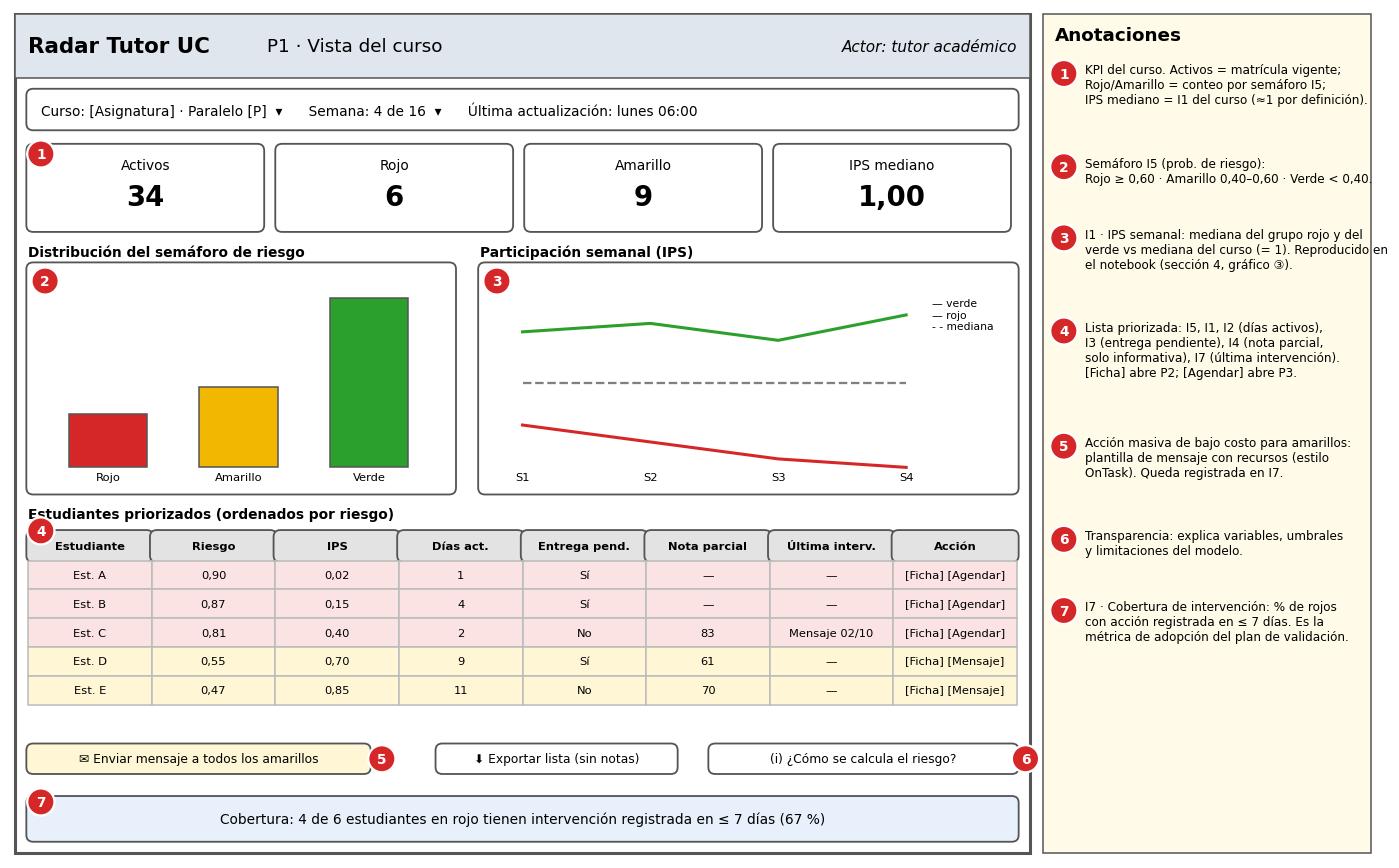
\includegraphics[width=\linewidth]{img/P1_vista_curso.png}\\[6pt]
\raggedright\scriptsize\color{gris}
\faFlask\ \ Datos públicos OULAD (22 cursos, 28\,785 estudiantes). Modelo entrenado con 2013 y probado con 2014. Curso AAA-2014J al cerrar la semana 4.
\end{column}
\begin{column}{0.65\textwidth}
\centering{\footnotesize\bfseries\color{gris} Pantalla P1 construida en el notebook}\\[3pt]
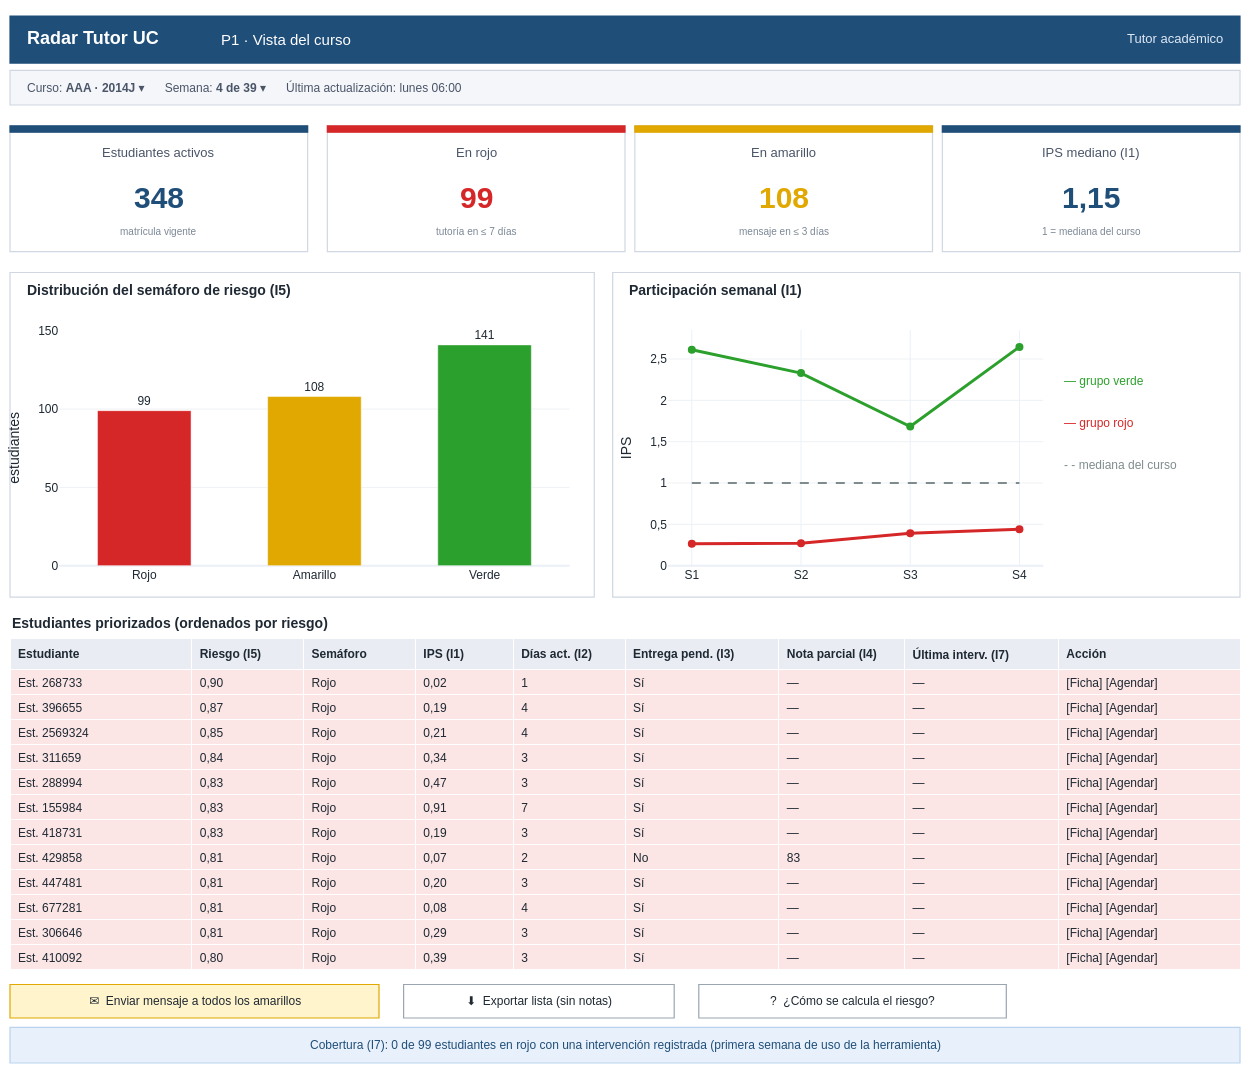
\includegraphics[height=6.3cm]{img/app_P1.png}
\end{column}
\end{columns}
\end{frame}

\begin{frame}{La ficha explica por qué un estudiante está en alerta}
\begin{columns}[c]
\begin{column}{0.62\textwidth}
\centering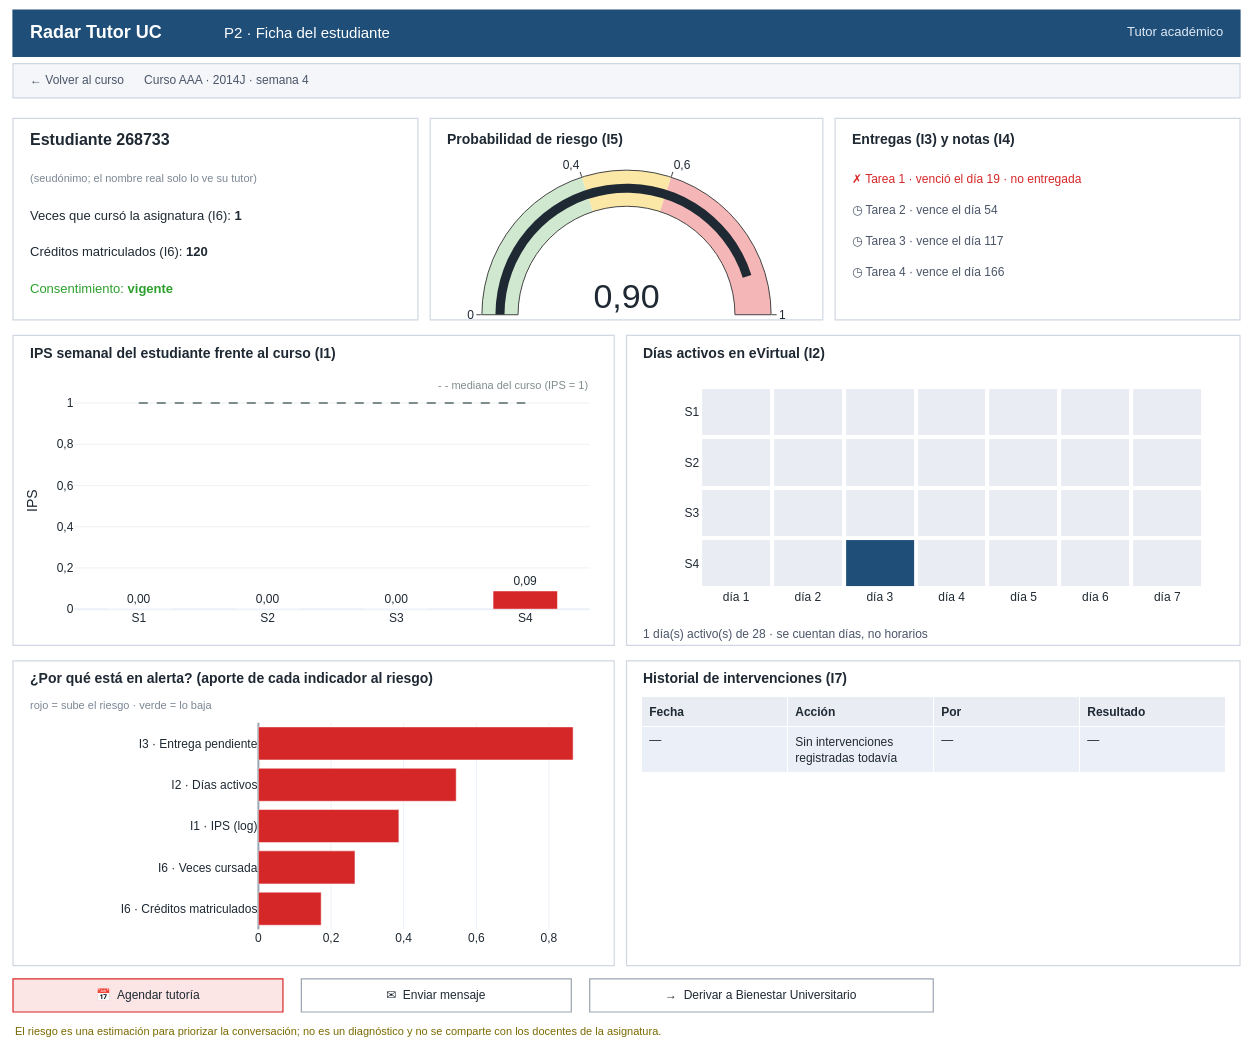
\includegraphics[height=6.6cm]{img/app_P2.png}
\end{column}
\begin{column}{0.36\textwidth}
\small
\begin{itemize}
\item Riesgo de \textbf{0,90}: un solo día activo en cuatro semanas y una tarea vencida sin entregar.
\item El gráfico \emph{¿Por qué está en alerta?} muestra cuánto aporta cada indicador.
\item Desde aquí el tutor \textbf{agenda la tutoría}, y queda registrada para la validación.
\end{itemize}
\end{column}
\end{columns}
\end{frame}

\begin{frame}{¿Qué tan bien funciona?}
\begin{columns}[c]
\begin{column}{0.64\textwidth}
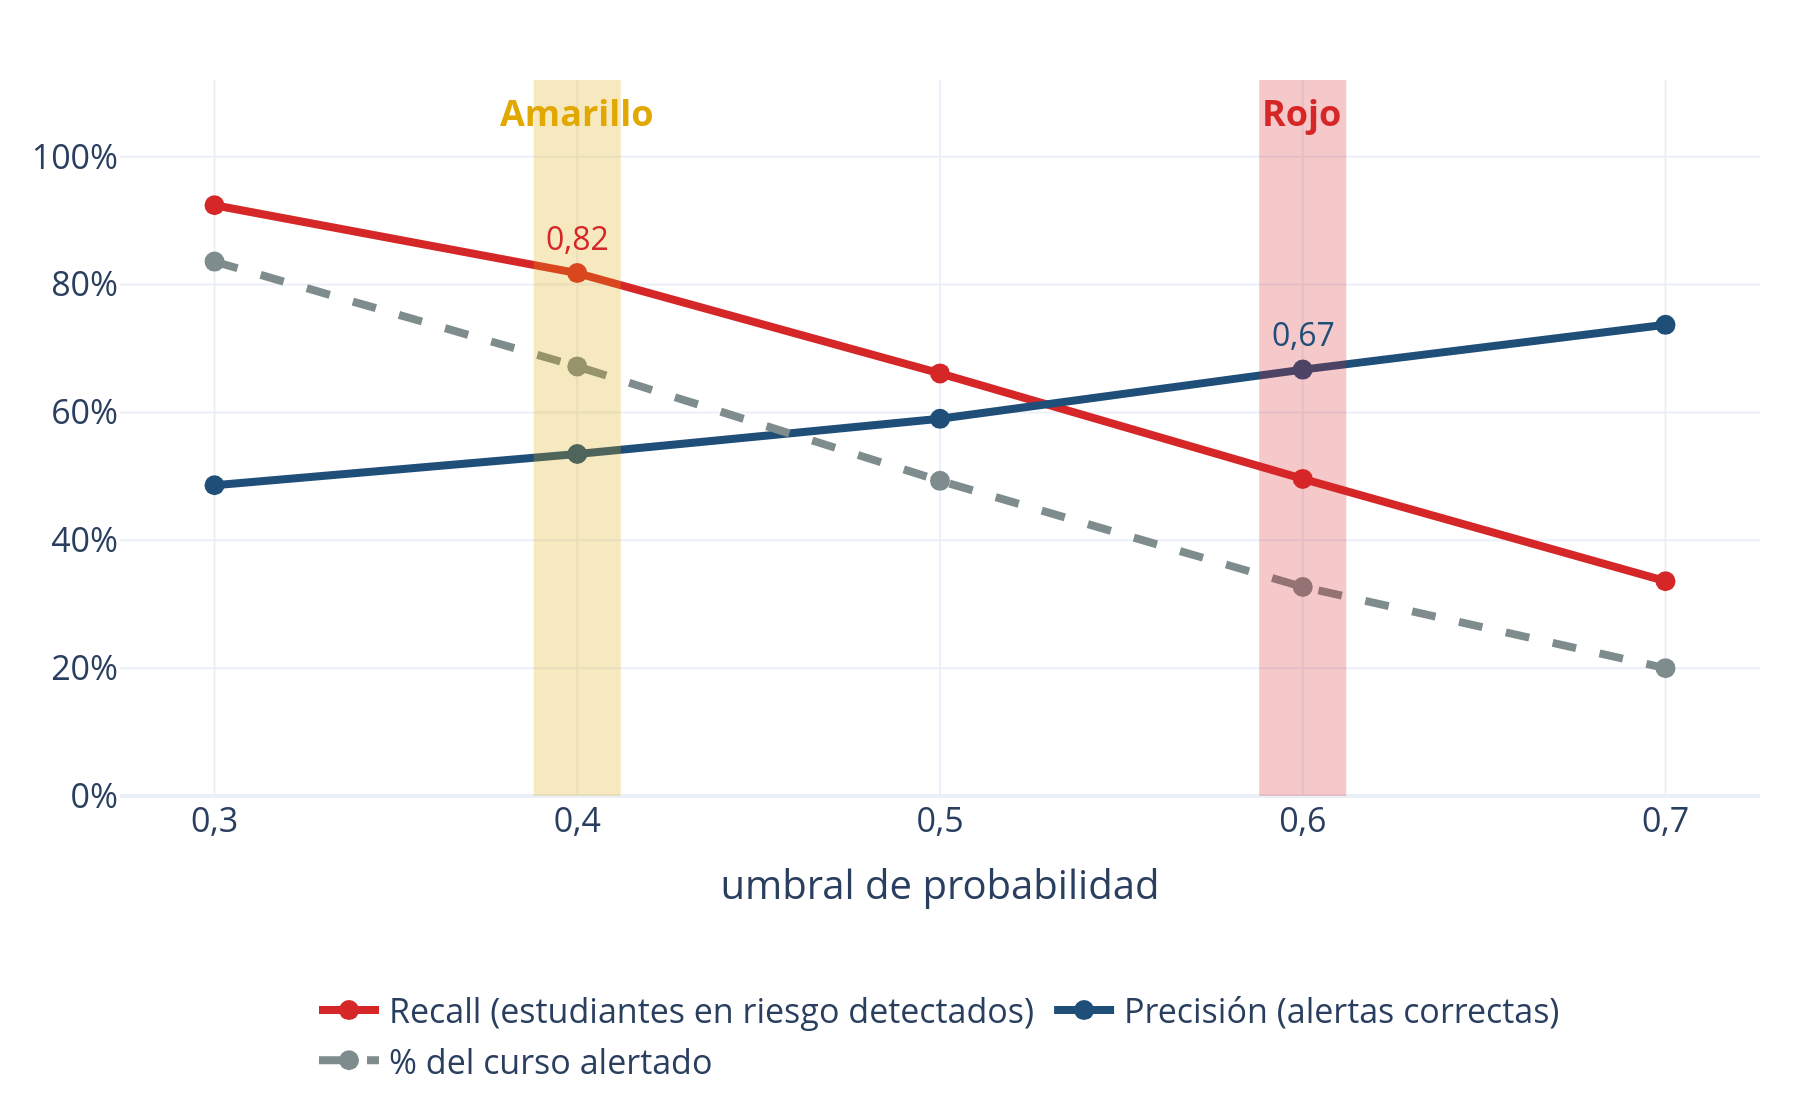
\includegraphics[width=\linewidth]{img/metricas_pitch.png}
\end{column}
\begin{column}{0.34\textwidth}
\dato{azul}{0,72}{AUC en la cohorte de prueba (2014)}
\vspace{2pt}
\dato{rojo}{82 de 100}{estudiantes en riesgo detectados en la semana 4}
\vspace{1pt}
\footnotesize
\begin{itemize}
\item En rojo, \textbf{2 de cada 3} alertas son correctas.
\item Sirve para \textbf{priorizar}, no para etiquetar.
\end{itemize}
\end{column}
\end{columns}
\end{frame}

% =====================================================================
\setbloque{4 · Validación y preguntas abiertas · 2 min}
\begin{frame}{Lo que el prototipo todavía no puede decir}
\begin{columns}[T]
\begin{column}{0.48\textwidth}
\begin{tarjeta}[\faExclamationTriangle\ \ Limitaciones]{ambar}\small
\begin{itemize}
\item No son datos de la UCuenca: habría que recalibrar con eVirtual.
\item Un umbral único no sirve para todos los cursos (del 10\,\% al 72\,\% en rojo).
\item Predecir no demuestra que la tutoría \textbf{cambie} el resultado.
\end{itemize}
\end{tarjeta}
\end{column}
\begin{column}{0.48\textwidth}
\begin{tarjeta}[\faBalanceScale\ \ Revisión de sesgos]{rojo}\small
\begin{itemize}
\item Recall de \textbf{0,77} en estudiantes de 35 a 55 años frente a \textbf{0,84} en menores de 35.
\item AUC de 0,69 en mujeres y 0,73 en hombres.
\item ¿Son diferencias reales o azar? Todavía no lo sabemos.
\end{itemize}
\end{tarjeta}
\end{column}
\end{columns}
\end{frame}

\begin{frame}{Plan de validación en tres niveles}
\begin{columns}[T]
\begin{column}{0.32\textwidth}
\begin{tarjeta}[\faCogs\ \ Técnica]{azul}\footnotesize
\emph{¿Mide lo que dice medir?}\\[4pt]
Validación temporal con cohortes anteriores de la UCuenca.\\[3pt]
Éxito: AUC ≥ 0,70, recall ≥ 0,75 y brecha entre grupos ≤ 0,05.
\end{tarjeta}
\end{column}
\begin{column}{0.32\textwidth}
\begin{tarjeta}[\faGraduationCap\ \ Pedagógica]{rojo}\footnotesize
\emph{¿Cambia algo en el aprendizaje?}\\[4pt]
\textbf{H1:} los alertados aprueban más si su tutor usa la herramienta.\\[3pt]
Sorteo por paralelo, un semestre, variable aprobado / no aprobado. Unos 356 alertados por grupo.
\end{tarjeta}
\end{column}
\begin{column}{0.32\textwidth}
\begin{tarjeta}[\faUsers\ \ Usabilidad y adopción]{verde}\footnotesize
\emph{¿La entienden y la usan?}\\[4pt]
SUS, entrevistas y registro de uso con 6 a 10 tutores.\\[3pt]
Éxito: SUS ≥ 68, 70\,\% de uso semanal, 80\,\% de rojos atendidos a tiempo.
\end{tarjeta}
\end{column}
\end{columns}
\end{frame}

\begin{frame}{Preguntas que todavía no sabemos responder}
\begin{enumerate}
\setlength{\itemsep}{5pt}
\item Si el grupo con herramienta aprueba un 66\,\% y el otro un 60\,\%, ¿la diferencia es real o es azar?
\item ¿Cuántos paralelos necesitamos si sorteamos paralelos y no estudiantes?
\item Nuestra variable es aprobado / no aprobado: ¿qué prueba estadística usamos?
\item ¿Cuál es el intervalo de confianza del recall (0,82) y del AUC (0,72)?
\item ¿La diferencia de recall por edad (0,77 frente a 0,84) es significativa?
\end{enumerate}
\end{frame}

% =====================================================================
{\setbeamertemplate{footline}{}
\begin{frame}
\begin{tikzpicture}[remember picture,overlay]
  \fill[azul] (current page.north west) rectangle (current page.south east);
  \node[text=white,font=\fontsize{34}{36}\selectfont\bfseries] at ([yshift=1.2cm]current page.center) {Gracias};
  \node[text=white!80!azul,font=\large,align=center] at ([yshift=-0.2cm]current page.center) {¿Preguntas?};
  \node[text=white!70!azul,font=\small,align=center] at ([yshift=-1.8cm]current page.center)
    {Del aviso tardío del primer parcial a una alerta en la semana 4 que se puede validar.};
\end{tikzpicture}
\end{frame}}

\setbloque{}
\begin{frame}{Referencias}
\scriptsize
\begin{itemize}
\setlength{\itemsep}{3pt}
\item Aguilar, B., Maldonado-Mahauad, J. y Sigua, E. (2021). \emph{FlipMyLearning: A tool for monitoring and predicting learner behavior in Moodle}.
\item Asamblea Nacional del Ecuador (2021). \emph{Ley Orgánica de Protección de Datos Personales}. Registro Oficial, Quinto Suplemento n.º 459.
\item Bravo Guerrero, F., Peña Ortega, M. e Illescas Peña, L. (2020). Reprobación y abandono de estudiantes universitarios. \emph{Uniandes EPISTEME}, 7(4), 502--516.
\item Brooke, J. (1996). SUS: A ``quick and dirty'' usability scale. En P. W. Jordan et al. (Eds.), \emph{Usability Evaluation in Industry} (pp. 189--194). Taylor \& Francis.
\item Guerra, J. et al. (2020). Adaptation and evaluation of a learning analytics dashboard to improve academic support at three Latin American universities. \emph{British Journal of Educational Technology}, 51(4), 973--1001.
\item Kuzilek, J., Hlosta, M. y Zdrahal, Z. (2017). Open University Learning Analytics dataset. \emph{Scientific Data}, 4, 170171.
\item Proyecto LALA (2020--2021). \emph{Boletín informativo} n.º 3, 4 y 5.
\end{itemize}
\end{frame}

\end{document}
